\documentclass{article}
\usepackage[left=3cm,right=3cm,top=2cm,bottom=2cm]{geometry}
\usepackage{makeidx}         % allows index generation
\usepackage[pdftex]{graphicx,color}          % standard LaTeX graphics tool
\DeclareGraphicsRule{.pdftex}{pdf}{.pdftex}{}
                             % when including figure files
\usepackage{multicol}        % used for the two-column index
\usepackage[bottom]{footmisc}% places footnotes at page bottom

\usepackage{booktabs}
\usepackage{arydshln}
\setlength\dashlinedash{0.5pt}
\setlength\dashlinegap{1.5pt}
\setlength\arrayrulewidth{0.3pt}

\usepackage{amssymb}
\usepackage{amsmath}
\usepackage{pifont}
\usepackage{bm}
\usepackage{cancel}
\usepackage{multirow}
\usepackage{amsmath}
\usepackage{epstopdf}
\usepackage[caption=false,font=footnotesize]{subfig}

\usepackage{listings}


\DeclareMathOperator*{\argmin}{arg\,min}

\DeclareGraphicsExtensions{.eps, .pdf, .png, .jpg}
\graphicspath{{./images/Ex1/}, {./images/Ex2/}, {./images/Ex3/}, {./images/Ex4/}, {./images/Ex5/}, {./images/Ex6/},{./}}

\newcommand{\red}[1]{{\color{red}#1}}
\renewcommand{\vec}[1]{\bm{#1}}
\newcommand{\mat}[1]{\bm{#1}}
\newcommand{\cframe}[1]{$\langle #1 \rangle$}
\newcommand{\prescript}[2]{\phantom{}^{#1}_{#2}}

\newcommand\frontmatter{%
    \cleardoublepage
%%  \@mainmatterfalse
  \pagenumbering{roman}}
\newcommand\mainmatter{%
    \cleardoublepage
%%  \@mainmattertrue
  \pagenumbering{arabic}}
%%%%%%%%%%%%%%%%%%%%%%%%%%%%%%%%%%%%%%%%%%%%%%%%%%%%%%%%%%%%%%%%%%%%%

\begin{document}
\frontmatter
\onecolumn
\vskip 1cm
%\pagestyle{empty}
\begin{center}
\huge \textsc{Cooperative Robotics}\\
\vskip 1cm

\skip 0.5cm

\vskip 5cm

\normalsize
Authors: Piccinini Davide, Porta Francesco and Gotelli Andrea
EMAILs: 4343879@studenti.unige.it, 4404040@studenti.unige.it
Date: 21/12/2020
\end{center}
\clearpage
\mainmatter
\section*{General notes}

\begin{itemize}
	\item Exercises 1-4 are done with the ROBUST matlab main and unity visualization tools. Exercises 5-6 are done with the DexROV matlab main and unity visualization tools.
	\item Comment and discuss the simulations, in a concise scientific manner. Further comments, other than the questions, can be added, although there is no need to write 10 pages for each exercise.
	\item Aid the discussion with screenshots of the simulated environment (compress them to maintain a small overall file size), and graphs of the relevant variables (i.e. activation functions of inequality tasks, task variables, and so on). Graphs should always report the units of measure in both axes, and legends whenever relevant.
	\item Report the thresholds whenever relevant.
	\item Report the mathematical formula employed to derive the task jacobians and the control laws when asked, including where they are projected.
	\item If needed, part of the code can be inserted as a discussion reference.
\end{itemize}


Use the following template when you need to discuss the hierarchy of tasks of a given action or set of actions:
\begin{table}[htb]
	\caption{Example of actions/hierarchy table: a number in a given cell represents the priority of the control task (row) in the hierarchy of the control action (column). The type column indicates whether the objective is an equality (E) or inequality (I) one.}
	\label{tbl:actions_table}
	\begin{center}
		\footnotesize
		\begin{tabular}{ccccc}
			\toprule
			Task & Type & $\mathcal{A}_{1}$ & $\mathcal{A}_{2}$ & $\mathcal{A}_{3} $	 \\
			\midrule
			Task A                    & I & 1 &   & 1  \\
			\hdashline
			Task B                & I & 2 & 1 &   \\
			\hdashline
			Task C                       & E &   & 2 & 2   \\

			\bottomrule
		\end{tabular}
	\end{center}
\end{table}% %

\clearpage


\section{Exercise 1: Implement a “Safe Waypoint Navigation” Action.}

\subsection{Adding a vehicle position control objective}
Initialize the vehicle far away from the seafloor. An example position could be
\begin{displaymath}
\begin{bmatrix} 10.5 & 35.5 & -36 & 0 & 0 & \pi/2\end{bmatrix}^\top
\end{displaymath} 
Give a target position that is also sufficiently away from the seafloor, e.g.,
\begin{displaymath}
\begin{bmatrix} 10.5 & 37.5 & -38 & 0 & 0 & 0 \end{bmatrix}^\top
\end{displaymath}

Goal: Implement a vehicle position control task, and test that the vehicle reaches the required position and orientation.


\subsubsection{Q1: What is the Jacobian relationship for the Vehicle Position control task? How was the task reference computed?}
The Jacobian relationship for the Vehicle Position control task need to take into account the linear velocities of the vehicle. In the configuration vector y the velocities are expressed in the vehicle frame so the Jacobian has to project them in the reference frame. In fact, the task reference was computed taking into account the position of the goal and the vehicle expressed in the reference frame.


\subsubsection{Q2: What is the behaviour if the Horizontal Attitude is enabled or not? Try changing the initial or target orientation in terms of roll and pitch angles. Discuss the behaviour.}


\subsubsection{Q3: Swap the priorities between Horizontal Attitude and the Vehicle Position control task. Discuss the behaviour.}

\subsubsection{Q4: What is the behaviour if the Tool Position control task is active and what if it is disabled? Which of the settings should be used for a Safe Waypoint Navigation action? Report the final hierarchy of tasks (and their priorities, see the template table in the introduction) which makes up the Safe Waypoint Navigation action.}


\subsection{Adding a safety minimum altitude control objective}
Initialize the vehicle at the position:
\begin{displaymath}
\begin{bmatrix} 48.5 & 11.5 & -33 & 0 & 0 &-\pi/2\end{bmatrix}^\top
\end{displaymath}
Choose as target point for the vehicle position the following one:
\begin{displaymath}
\begin{bmatrix} 50 & -12.5 & -33 & 0 & 0 & -\pi/2 \end{bmatrix}^\top
\end{displaymath}

Goal: Implement a task to control the altitude from the seafloor. Check that at all times the minimum distance from the seafloor is guaranteed.


\subsubsection{Q1: Report the new hierarchy of tasks of the Safe Waypoint Navigation and their priorities. Comment how you choose the priority level for the minimum altitude.}

\subsubsection{Q2: What is the Jacobian relationship for the Minimum Altitude control task? Report the formula for the desired task reference generation, and the activation thresholds.}

\subsubsection{Q3: Try imposing a minimum altitude of 1, 5, 10 m respectively. What is the behaviour? Does the vehicle reach its final goal in all cases?}

\subsubsection{Q4: How was the sensor distance processed to obtain the altitude measurement? Does it work in all cases or some underlying assumptions are implicitly made?}

\clearpage

\section{Exercise 2: Implement a Basic “Landing” Action.}
\subsection{Adding an altitude control objective}
Initialize the vehicle at the position:
\begin{displaymath}
\begin{bmatrix} 10.5 & 37.5 & -38 & 0 & -0.06 & 0.5 \end{bmatrix}^\top
\end{displaymath}

Goal: add a control task to regulate the altitude to zero.

\subsubsection{Q1: Report the hierarchy of task used and their priorities to implement the Landing Action. Comment how you choose the priority level for the altitude control task.}

\subsubsection{Q2: What is the Jacobian relationship for the Altitude control task? How was the task reference computed?}

\subsubsection{Q3: how does this task differs from a minimum altitude control task?}

\subsection{Adding mission phases and change of action}
Initialize the vehicle at the position:
\begin{displaymath}
\begin{bmatrix} 8.5 & 38.5 & -36 & 0 & -0.06 & 0.5 \end{bmatrix}^\top
\end{displaymath}
Use a "safe waypoint navigation action" to reach the following position:
\begin{displaymath}
\begin{bmatrix} 10.5 & 37.5 & -38 & 0 & -0.06 & 0.5 \end{bmatrix}^\top
\end{displaymath}
When the position has been reached, land on the seafloor using the basic "landing" action.

\subsubsection{Q1: Report the unified hierarchy of tasks used and their priorities.}

\subsubsection{Q2: How did you implement the transition from one action to the other?}

\clearpage

\section{Exercise 3: Improve the “Landing” Action}
\subsection{Adding an alignment to target control objective}
If we use the landing action, there is no guarantee that we land in from of the nodule/rock. We need to add additional constraints to make the vehicle face the nodule. The position of the rock is contained in the variable \texttt{rock\_center}.

Initialize the vehicle at the position:
\begin{displaymath}
\begin{bmatrix} 8.5 & 38.5 & -36 & 0 & -0.06 & 0.5 \end{bmatrix}^\top
\end{displaymath}
Use a "safe waypoint navigation action" to reach the following position:
\begin{displaymath}
\begin{bmatrix} 10.5 & 37.5 & -38 & 0 & -0.06 & 0.5 \end{bmatrix}^\top
\end{displaymath}
Then land, aligning to the nodule.

Goal: Add an alignment task between the longitudinal axis of the vehicle ($x$ axis) and the nodule target. In particular, the $x$ axis of the vehicle should align to the projection, on the inertial horizontal plane, of the unit vector joining the vehicle frame to the nodule frame.

\subsubsection{Q1: Report the hierarchy of tasks used and their priorities in each action. Comment the behaviour.}

\subsubsection{Q2: What is the Jacobian relationship for the Alignment to Target control task? How was the task reference computed?}

\subsubsection{Q3: Try changing the gain of the alignment task. Try at least three different values, where one is very small. What is the observed behaviour? Could you devise a solution that is gain-independent guaranteeing that the landing is accomplished aligned to the target?}

\subsubsection{Q4: After the landing is accomplished, what happens if you try to move the end-effector? Is the distance to the nodule sufficient to reach it with the end-effector? Comment the observed behaviour. If, after landing, the nodule is not in the manipulator's workspace, how would you solve this problem to guarantee it?}


\clearpage
\section{Exercise 4: Implementing a Fixed-base Manipulation Action}
\subsection{Adding non-reactive tasks}
To manipulate as a fixed based manipulator, we need to constraint the vehicle to not move, otherwise the tool frame position task will make the vehicle move.

Goal: Add a constraint task that fixes the vehicle velocity to zero. Land on the seafloor. Try reaching the rock position with the end-effector, and observe that the vehicle does not move.

\subsubsection{Q1: Report the hierarchy of tasks used and their priorities in each action. At which priority level did you add the constraint task?}

\subsubsection{Q2: What is the Jacobian relationship for the Vehicle Null Velocity task? How was the task reference computed?}

\subsubsection{Q3: Suppose that the vehicle is floating, i.e. not landed on the seafloor. What would happen, if due to currents, the vehicle moves?}


\subsection{Adding a joint limit task}
Let us now constrain the arm with the actual joint limits. The vector variables \texttt{uvms.jlmin} and \texttt{uvms.jlmax} contain the maximum and minimum values respectively.

Goal: Add a joint limits avoidance task. Land on the seafloor. Try reaching the rock position with the end-effector, and observe that the vehicle does not move and that all the joints are within their limits.

\subsubsection{Q1: Report the hierarchy of tasks used and their priorities in each action. At which priority level did you add the joint limits task?}

\subsubsection{Q2: What is the Jacobian relationship for the Joint Limits task? How was the task reference computed?}

\clearpage
\section{Exercise 5: Floating Manipulation}
\subsection{Adding an optimization control objective}
Use the DexROV simulation for this exercise.

The goal is to try to optimize the joint positions, if possible, to keep the first four joints in a "preferred shape", represented by the following vector
\begin{displaymath}
\begin{bmatrix}-0.0031 & 1.2586 & 0.0128 & -1.2460 \end{bmatrix}^\top
\end{displaymath}

Goal: Add an optimization objective to keep the first four joints of the manipulator in the preferred shape. Observe the behaviour with and without the task

\subsubsection{Q1: Report the hierarchy of tasks used and their priorities in each action. At which priority level did you add the optimization task?}

\subsubsection{Q2: What is the Jacobian relationship for the Joint Preferred Shape task? How was the task reference computed?}

\subsubsection{Q3: What is the difference between having or not having this objective?}

\subsection{Adding mission phases}
Let us now structure the mission in more than one phase. In the first phase, exploit the previous exercises, and implement a safe waypoint navigation. Move the vehicle to a location close to the current defined end-effector goal position, just slightly above it. Then, trigger a change of action and perform floating manipulation.

Goal: introduce mission phases in the floating manipulation scenario. Observe the difference.

\subsubsection{Q1: Report the unified hierarchy of tasks used and their priorities. Which task is active in which phase/action?}

\subsubsection{Q2: What is the difference with the previous simulation (still in exercise 5), where only one action was used?}

\clearpage
\section{Exercise 6: Floating Manipulation with Arm-Vehicle Coordination Scheme}
\subsection{Adding the parallel arm-vehicle coordination scheme}
Let us now see how the two different subsystems (arm and vehicle) can be properly coordinate. Introduce in the simulation a sinusoidal velocity disturbance acting on the vehicle, and assume the actual vehicle velocity measurable. To do so, add a constant (in the inertial frame) velocity vector to the reference vehicle velocity before integrating it in the simulator.

Goal: modify the control part to implement the parallel arm-vehicle coordination scheme. Observe that, even with a disturbance acting on the vehicle, the end-effector can stay in the required constant position.

\subsubsection{Q1: Which tasks did you introduce to implement the parallel coordination scheme?}
In order to obtain the desired behavior we have introduced two kinds of disturbances, one linear and the other as angular velocity disturbance, expressed in the inertial frame. The vehicle suffers from these velocities, as they are added before integration. 
\begin{lstlisting}
%	Adding the disturbances
disturb = [0 0.025 0]';
disturb_ang = [0 0 0]';
disturb_ang = disturb_ang*0.5*sin(0.5*t*2*pi);
uvms.p_dot(1:3) = uvms.wTv(1:3,1:3)*disturb;
uvms.p_dot(4:6) = uvms.wTv(1:3,1:3)*disturb_ang;
    
% beware: p_dot should be projected on <v>
uvms.p = integrate_vehicle(uvms.p, uvms.p_dot, deltat);
\end{lstlisting}

In order to cope 


\subsubsection{Q2: Show the plot of the position of the end-effector, showing that it is constant. Show also a plot of the velocities of the vehicle and of the arm.}
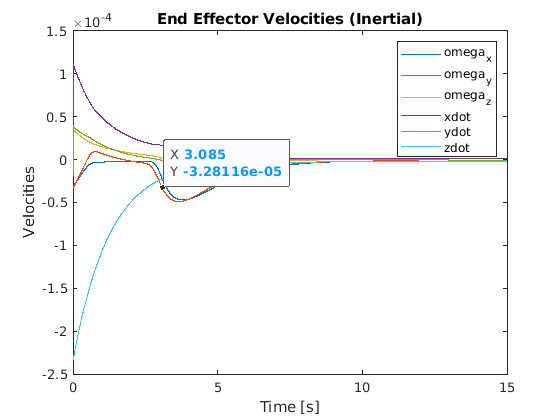
\includegraphics{EE_velocities}
\subsubsection{Q3: What happens if the sinusoidal disturbance becomes too big? Try increasing the saturation value of the end-effector task if it is too low.}



%\begin{figure}[t]
%	\centering
%	\subfloat[]{\includegraphics[height=7cm]{trident.jpg}}\label{fig:trident}
%	\subfloat[]{\includegraphics[height=7cm]{maris.jpg}}\label{fig:maris}
%	\caption{(a) TRIDENT UVMS (b) MARIS UVMS.}\label{fig:uvms_examples}
%\end{figure}



%		\begin{figure}[b]
%			\centering
%			\subfloat[]{\frame{\includegraphics[keepaspectratio,height=3cm]{trident1.eps}}}
%			\subfloat[]{\frame{\includegraphics[keepaspectratio,height=3cm]{trident2.eps}}}
%			\subfloat[]{\frame{\includegraphics[keepaspectratio,height=3cm]{trident3.eps}}}
%			\subfloat[]{\frame{\includegraphics[keepaspectratio,height=3cm]{trident4.eps}}}
%			\caption{Sequence of snapshots taken from the onboard camera during the TRIDENT final experiments.}
%			\label{fig_tri_trial_maiorca_img}
%		\end{figure}


\end{document}
